\documentclass[journal,12pt,twocolumn]{IEEEtran}
%
\usepackage{setspace}
\usepackage{textcomp}
\usepackage{gensymb}
%\doublespacing
\singlespacing

\usepackage[cmex10]{amsmath}
\usepackage{amsthm}
%\usepackage{iithtlc}
\usepackage{mathrsfs}
\usepackage{txfonts}
\usepackage{stfloats}
\usepackage{bm}
\usepackage{cite}
\usepackage{cases}
\usepackage{subfig}
%\usepackage{xtab}
\usepackage{longtable}
\usepackage{multirow}
%\usepackage{algorithm}
%\usepackage{algpseudocode}
\usepackage{enumitem}
\usepackage{mathtools}
\usepackage{steinmetz}
\usepackage{tikz}
\usepackage{circuitikz}
\usepackage{verbatim}
\usepackage{tfrupee}
\usepackage[breaklinks=true]{hyperref}
%\usepackage{stmaryrd}
\usepackage{tkz-euclide} % loads  TikZ and tkz-base
%\usetkzobj{all}
\usetikzlibrary{calc,math}
\usepackage{listings}
    \usepackage{color}                                            %%
    \usepackage{array}                                            %%
    \usepackage{longtable}                                        %%
    \usepackage{calc}                                             %%
    \usepackage{multirow}                                         %%
    \usepackage{hhline}                                           %%
    \usepackage{ifthen}                                           %%
  %optionally (for landscape tables embedded in another document): %%
    \usepackage{lscape}     
\usepackage{multicol}
\usepackage{chngcntr}
%\usepackage{enumerate}

%\usepackage{wasysym}
%\newcounter{MYtempeqncnt}
\DeclareMathOperator*{\Res}{Res}
%\renewcommand{\baselinestretch}{2}
\renewcommand\thesection{\arabic{section}}
\renewcommand\thesubsection{\thesection.\arabic{subsection}}
\renewcommand\thesubsubsection{\thesubsection.\arabic{subsubsection}}

\renewcommand\thesectiondis{\arabic{section}}
\renewcommand\thesubsectiondis{\thesectiondis.\arabic{subsection}}
\renewcommand\thesubsubsectiondis{\thesubsectiondis.\arabic{subsubsection}}

% correct bad hyphenation here
\hyphenation{op-tical net-works semi-conduc-tor}
\def\inputGnumericTable{}                                 %%

\lstset{
%language=C,
frame=single, 
breaklines=true,
columns=fullflexible
}
\newenvironment{amatrix}[1]{%
  \left(\begin{array}{@{}*{#1}{c}|c@{}}
}{%
  \end{array}\right)
}
\DeclarePairedDelimiter\abs{\lvert}{\rvert}%
\DeclarePairedDelimiter\norm{\lVert}{\rVert}%

% Swap the definition of \abs* and \norm*, so that \abs
% and \norm resizes the size of the brackets, and the 
% starred version does not.
\makeatletter
\let\oldabs\abs
\def\abs{\@ifstar{\oldabs}{\oldabs*}}
%
\let\oldnorm\norm
\def\norm{\@ifstar{\oldnorm}{\oldnorm*}}
\makeatother

\newtheorem{theorem}{Theorem}[section]
\newtheorem{problem}{Problem}
\newtheorem{proposition}{Proposition}[section]
\newtheorem{lemma}{Lemma}[section]
\newtheorem{corollary}[theorem]{Corollary}
\newtheorem{example}{Example}[section]
\newtheorem{definition}[problem]{Definition}
%\newtheorem{thm}{Theorem}[section] 
%\newtheorem{defn}[thm]{Definition}
%\newtheorem{algorithm}{Algorithm}[section]
%\newtheorem{cor}{Corollary}
\newcommand{\BEQA}{\begin{eqnarray}}
\newcommand{\EEQA}{\end{eqnarray}}
\newcommand{\define}{\stackrel{\triangle}{=}}
\bibliographystyle{IEEEtran}
%\bibliographystyle{ieeetr}
\providecommand{\mbf}{\mathbf}
\providecommand{\pr}[1]{\ensuremath{\Pr\left(#1\right)}}
\providecommand{\qfunc}[1]{\ensuremath{Q\left(#1\right)}}
\providecommand{\sbrak}[1]{\ensuremath{{}\left[#1\right]}}
\providecommand{\lsbrak}[1]{\ensuremath{{}\left[#1\right.}}
\providecommand{\rsbrak}[1]{\ensuremath{{}\left.#1\right]}}
\providecommand{\brak}[1]{\ensuremath{\left(#1\right)}}
\providecommand{\lbrak}[1]{\ensuremath{\left(#1\right.}}
\providecommand{\rbrak}[1]{\ensuremath{\left.#1\right)}}
\providecommand{\cbrak}[1]{\ensuremath{\left\{#1\right\}}}
\providecommand{\lcbrak}[1]{\ensuremath{\left\{#1\right.}}
\providecommand{\rcbrak}[1]{\ensuremath{\left.#1\right\}}}
\providecommand{\system}{\overset{\mathcal{H}}{ \longleftrightarrow}}
	%\newcommand{\solution}[2]{\textbf{Solution:}{#1}}
\newcommand{\solution}{\noindent \textbf{Solution: }}
\newcommand{\cosec}{\,\text{cosec}\,}
\providecommand{\dec}[2]{\ensuremath{\overset{#1}{\underset{#2}{\gtrless}}}}
\newcommand{\myvec}[1]{\ensuremath{\begin{pmatrix}#1\end{pmatrix}}}
\newcommand{\mydet}[1]{\ensuremath{\begin{vmatrix}#1\end{vmatrix}}}
%\numberwithin{equation}{section}
\numberwithin{equation}{subsection}
%\numberwithin{problem}{section}
%\numberwithin{definition}{section}
\makeatletter
\@addtoreset{figure}{problem}
\makeatother
\let\StandardTheFigure\thefigure
\let\vec\mathbf
\usepackage{mathtools, nccmath}
\begin{document}
\begin{center}
\huge Assignment 3\\
\large SUBHASISH SAIKIA\\
\large AI20MTECH14001\\
\end{center}
\vspace{0.5cm}
\begin{abstract}
This document explains the equation of a straight line, making an angle with the x-axis and passing through a given point.
\end{abstract}
\vspace{0.5cm}
Download all python codes from 
\begin{lstlisting}
https://github.com/subhasishsaikia22/EE5609-Matrix-theory
\end{lstlisting}
%
and latex-tikz codes from 
\begin{lstlisting}
https://github.com/subhasishsaikia22/EE5609-Matrix-theory
\end{lstlisting}
%
\vspace{0.5cm}
\section{Problem}
Find the equation of a straight line making an angle of 60$^{\circ}$
with OX and passing through the point $\myvec{2 \\-2}$. Transform the equation to the form 
\begin{align}
     \myvec{ cos\alpha \quad sin\alpha}x=p
\end{align} 

\section{Explanation}
Let the straight line pass through the point $\vec{A}=\myvec{2 \\-2}$ and makes an angle of 60$^{\circ}$ with x-axis.\\
So slope of the line, $m=\tan 60^{\circ}=\sqrt{3}$ and the direction vector  $\myvec{1 \\m} = \myvec{1 \\\sqrt{3}}$.\\\\
The vector form of the line passing through the point $\vec{A}=\myvec{2 \\-2}$ along the direction vector  $\myvec{1 \\\sqrt{3}}$ is given by:
\begin{align}
\vec{X}=\myvec{2 \\-2}+ \lambda_1\myvec{1 \\\sqrt{3}}
\end{align} 

The normal vector
\begin{align}
\vec{n}=\myvec{0 \quad -1\\1 \quad 0} \myvec{1 \\m} = \myvec{-\sqrt3\\ 1}
\end{align}
The equation of the line in terms of the normal vector is obtained as
\begin{align}
\vec{n^T}\myvec{x-A}  =0\\
\myvec{-\sqrt3\quad 1}x=\myvec{-\sqrt3\quad 1}A\\
\myvec{-\sqrt3\quad 1}x=\myvec{-\sqrt3\quad 1}\myvec{2 \\-2}\\
\myvec{-\sqrt3\quad 1}x=-2\sqrt{3}-2\\
\myvec{\sqrt3/2\quad -1/2}x=\sqrt{3}+1\\
\vspace{1cm}
\myvec{ cos 330^{\circ} \quad sin 330^{\circ}}x= 2.732
\end{align}

\begin{figure}[!]
 \begin{center}
  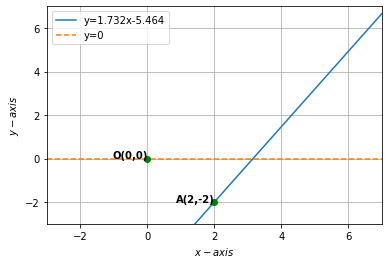
\includegraphics[width=10cm]{asignment 3/assignment3_fig.png}
    \caption{This is the 2D diagram of the straight line passing through $\myvec{2 \\-2}$ and at an angle of 60$^{\circ}$ with the x axis }
    \label{myfig:1}
    \end{center}
\end{figure}
\end{document}
